\newpage

\section{Tuesday, February 18, 2020}

Last time, we finished graph algorithms. Today, we'll begin \vocab{greedy algorithms}, which are a class of algorithms that repeatedly make ``locally optimal" decisions in an attempt to find a globally optimal solution.


\subsection{The Union-Find Data Structure}

Before we introduce Kruskal's algorithm, we'll need to first introduce a data structure known as the \vocab{union-find} or \vocab{disjoint-set} data structure. Why? Because this data structure is used in the implementation of Kruskal's algorithm, which is one of the two minimum spanning tree algorithms we will be talking about. \\

The union-find data structure consists of a collection of disjoint sets (i.e. a set of sets). Each disjoint set is uniquely determined by a \vocab{set representative}, which is some member of the set. In most applications, it doesn't actually matter which member of the set is used as the representative; all we care is that, if we ask for the representative of a set twice without making any modifications, we should get the same answer both times. \\

The union-find data structure supports the following operations:

\begin{enumerate}
    \item The \verb!MAKE-SET(x)! operation creates a new set whose only member is $x$. Since $x$ is the only member of this newly created set, $x$ must also be the representative of this set. Moreover, since we require the sets to be disjoint, we require that $x$ not already be in some other set.
    \item The \verb!UNION(x, y)! operation unites the two sets that contain the elements $x$ and $y$. More precisely, if $S_x$ and $S_y$ are the sets containing $x$ and $y$, then we remove both of these sets from our collection of sets, and we form a new set $S \defeq S_x \cup S_y$, which is subsequently added to the collection of sets. What element becomes the representative of the new set? Typically, if $S_x$ was originally larger than $S_y$, then we make the representative of $S_x$ the representative of $S$. Otherwise, we make the representative of $S_y$ the representative of $S$.
    \item The \verb!FIND-SET(x)! method takes in an element $x$ and returns the representative of the set containing $x$. Note that this means that \verb!FIND-SET(x)! might return \verb!x! itself (if \verb!x! is the representative of its set). 
\end{enumerate}


There are several applications of the union-find data structure. One of the many applications arises when we are trying to determine the connected components in an undirected graph. In particular, we can answer queries of the form ``Are vertices $u$ and $v$ in the same connected component?" with a quick running time by using this data structure. \\


Consider the following pseudocode: 


\vspace{1em}
\begin{center}
\line(1,0){400}
\end{center}

\begin{allintypewriter}
\# Input: A graph G.

\hspace{0cm}

\# Output: Nothing. This function is called as a preprocessing step 

\# in order to use the function SAME-COMPONENT(u, v).

\hspace{0.5cm}


CONNECTED-COMPONENTS(G) \string{ 

\hspace{0.5cm} for each vertex v $\in$ G \string{

\hspace{1cm} MAKE-SET(v) 

\hspace{0.5cm} \string}

\hspace{0.5cm} for each edge (u, v) $\in$ G \string{

\hspace{1cm} if FIND-SET(u) != FIND-SET(v) \string{

\hspace{1.5cm} UNION(u, v)

\hspace{1cm} \string}

\hspace{0.5cm} \string}

\string}

\hspace{0cm}

\# Input: Two vertices u and v. CONNECTED-COMPONENTS(G) must be 

\#  called prior to using this function.

\hspace{0cm}

\# Output: True if u and v are in the same connected component;

\# otherwise false. 

\hspace{0cm}

SAME-COMPONENT(u, v) \string{
    
    \hspace{0.5cm} return (FIND-SET(u) == FIND-SET(v))
    
\string}
\end{allintypewriter}

\begin{center}
\line(1,0){400}
\end{center}


How does these functions work?

\begin{itemize}
    \item We use a single union-find data structure that is initially empty. At first, we create a new disjoint set for each vertex. Each disjoint set in our union-find data structure will represent a connected component in our graph.
    \item Next, we traverse every edge in our graph $G$. For each edge $(u, v)$, we merge the two disjoint sets containing $u$ and $v$ (since they must be in the same component). 
    \item Finally, we can call the \verb!SAME-COMPONENT! function with two vertices $u$ and $v$ which simply compare the representatives of the sets $u$ and $v$ are in to determine whether the two vertices are in the same component.
\end{itemize}

\subsection{Implementation of the Union-Find Data Structure}

In our connected components example, we use a union-find data structure, but we never explain how the functions \verb!MAKE-SET!, \verb!UNION!, or \verb!FIND-SET! are implemented. In this section, we'll discuss how to implement these three methods. \\

Union-find data structures are typically implemented as a \vocab{disjoint-set forest} in which each member only points to its parent (the root of each tree is the representative of the disjoint set, and it is its own parent). The following figure from CLRS illustrates this idea:


\begin{figure}[h]
\centering
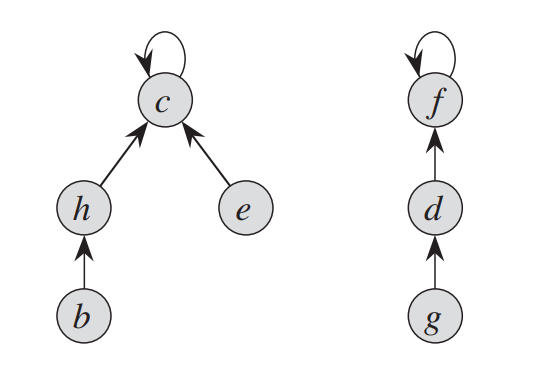
\includegraphics[scale=0.4]{media/ufds1}
\caption{A Disjoint Forest}
\end{figure}

The disjoint-set forest above represents the two sets $\{c, h, b, e\}$ with representative $c$ and $\{f, d, g\}$ with representative $f$. Note that the parent of any representative is itself. \\

How do we keep track of the parent of each vertex? This is easy --- we can just include an array called \verb!parent! as a part of our data structure implementation. For any vertex $v$, we can store the parent of $v$ in \verb!parent[v]!. \\

Now, we will discuss two heuristics to improve the running-time of various union-find operations. The first heuristic, known as the \vocab{union by rank heuristic}, is a heuristic that is applied when performing the \verb!UNION! operation. In particular, this heuristic specifies to make the root of the tree with fewer nodes to point to the root of the tree with more nodes.  Why? Because following the union by rank heuristic minimizes the overall depth of the resulting tree. \\


The following diagram illustrates the resulting tree that comes from performing the \verb!UNION! operation on two elements in the disjoint sets from the previous figure:
\newpage

\begin{figure}[h]
\centering
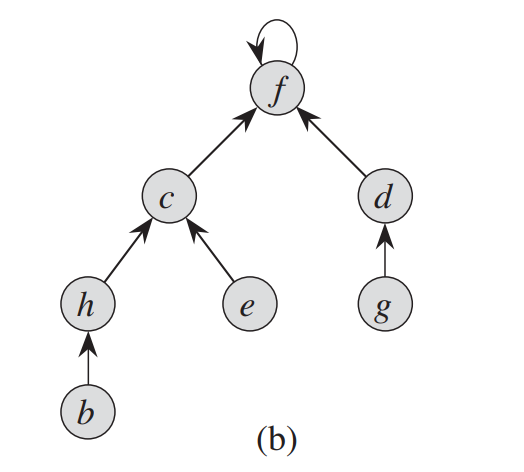
\includegraphics[scale=0.4]{media/ufds2}
\caption{Our Disjoint Forest after performing \texttt{UNION}}
\end{figure}

Note that $f$ is the representative of the resulting tree since we make the tree with fewer nodes point to the root of the tree with more nodes. \\

It would be computationally expensive to keep on recomputing the number of roots in each tree whenever we perform a \verb!UNION! operation. Thus, we can instead just maintain an array \verb!rank! which stores an upper bound on the height of each node. During a \verb!UNION! operation, we simply make the root with a smaller rank point to the root with the larger rank. \\


The second heuristic, known as \vocab{path compression} is a heuristic that is used during \verb!FIND-SET! operations to make each node on the find path point directly to the root. This technique is fairly easy to implement, and its purpose is to keep the depth of the tree small. \\


A C++ implementation of the union-find data structure is presented below:


\begin{lstlisting}
/* An implementation of the union-find data structure. */
class UnionFind {
    private:
        vector<int> parent;
        vector<int> rank;
    public:
        /* A constructor to initialize a union-find data structure with capacity N. */
        UnionFind(int N) {
            parent.assign(N, 0);
            rank.assign(N, 0);
            
            /* Each vertex is initially its own parent. */
            for (int i = 0; i < N; i++) {
                parent[i] = i;
            }
        }
    
    /* findSet(u) returns the representative of the set that u belongs to. */    
    int findSet(int u) {
        if (parent[u] == u) {
            /* u is the representative of its set. */
            return u;
        }
        /* Path compression heuristic. */
        parent[u] = findSet(parent[u]);
    }
    
    /* inSameSet(u, v) returns true if u and v are in the same set; false otherwise. */
    bool inSameSet(int u, int v) {
        /* We compare the set representatives. */
        return findSet(u) == findSet(v);
    }
    
    /* Union the sets that u and v belong in. */
    void unionSet(int u, int v) {
        if (!inSameSet(u, v)) {
            int rep1 = findSet(u);
            int rep2 = findSet(v);
            /* Union by rank heuristic. */
            if (rank[rep1] > rank[rep2]) {
                parent[rep2] = rep1;    
            } else {
                parent[rep1] = rep2;
                if (rank[rep1] == rank[rep2]) {
                    rank[rep2]++;
                }
            }
        }
    }

};
\end{lstlisting}


\subsection{Analysis of Union-Find Operations}

We won't derive 



\subsection{The Minimum Spanning Tree Problem}

The \vocab{minimum spanning tree} problem is stated below:




\subsubsection{Kruskal's Algorithm}

First, we'll discuss Kruskal's algorithm, which works by repeatedly finding a safe edge to add to the growing forest. In particular, this algorithm works by As stated in CLRS, ``Kruskal's algorithm qualifies as a greedy algorithm because, at each step, it adds to the forest an edge of least possible weight." \\

A 